Nesta seção será descrito o diagrama de máquina de estados, presente no SysML e também no UML. Ele é um diagrama comportamental que apresenta as mudanças de estado de uma certa entidade, indicando os eventos responsáveis pelas transições entre estados.

%\subsubsection{O que é o diagrama de máquinas de estados}
%texto

\subsubsection{Estrutura dos diagramas de máquinas de estado}
\begin{figure}[h]
\centering
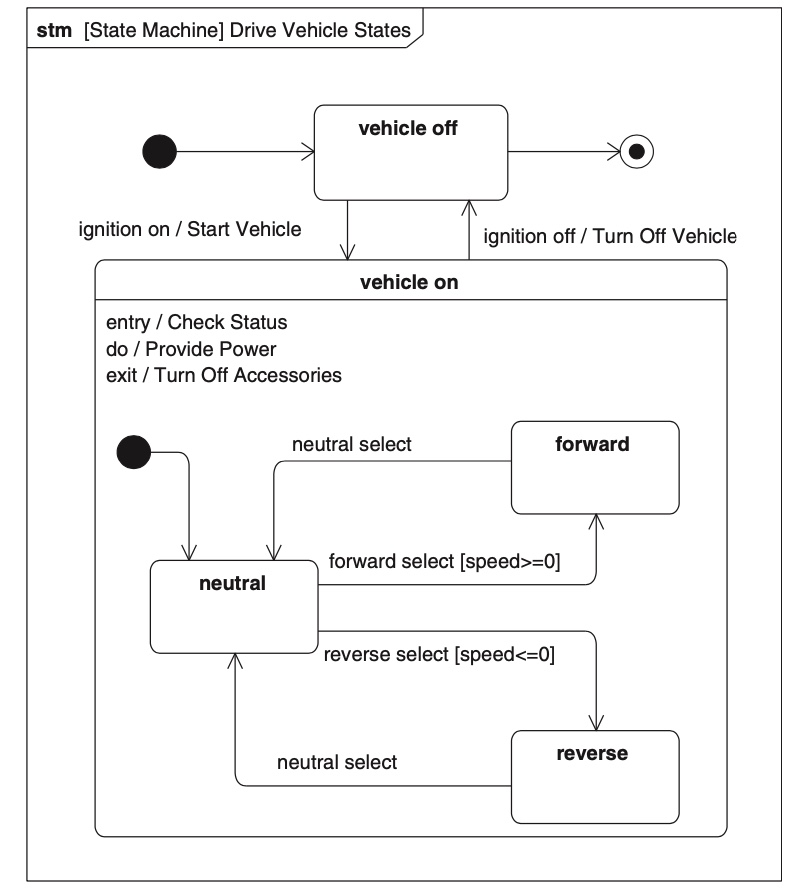
\includegraphics[width=0.75\textwidth]{figures/diagrama-maquina-estados.jpeg}
\caption{Diagrama Máquina de Estados}
\label{fig:state_machine_diagram}
\end{figure}
Na figura \ref{fig:state_machine_diagram}, pode-se observar os estados de um veículo, e também os estados quando o veículo está ligado, além dos eventos responsáveis pelas transições. 

Pode-se entender como estado a condição que determinada entidade permanece por um certo período. Já um evento é um acontecimento significativo bem determinado, no caso de máquina de estados, funcionando como gatilhos para a mudança de estado. Com essas duas definições, pode-se entender o funcionamento dos elementos do diagrama.

Como elementos importantes desse diagrama temos o círculo totalmente preenchido em preto e o círculo como outro menor dentro dele, representando, respectivamente, o estado inicial e o estado final. As setas representam as transições de estado e podem conter o evento causador dessa mudança. 

De maneira opcional, pode-se apresentar os comportamentos da entidade em determinado estado, podendo ser um comportamento realizado ao passar aquele estado, enquanto estiver nele ou ainda quando for transicionar para outro. Como pode ser observado no canto superior direito do estado do veículo ligado.

\subsubsection{Onde são utilizados com frequência}
Utilizado principalmente para descrever como um objeto muda de estado ao longo de seu tempo de vida, podendo ser uma maneira conveniente para apresentar objetos que sofrem muitas ações de diversos eventos ou ainda mostrar como certo objeto se comporta em certo caso de uso, mostrando o contexto de negócio, por exemplo. Considerando isso, permite auxiliar na modelagem de sistemas com muitas interações.